\documentclass[aspectratio=169]{beamer}
\usepackage[T1]{fontenc}
\usepackage[utf8]{inputenc}
\usepackage{lmodern}
\usepackage{microtype}
\usepackage{xcolor}
\usepackage{tikz}
\usetikzlibrary{positioning, arrows.meta, calc}
\usepackage{fontawesome5}
\definecolor{wurgreen}{HTML}{34B233}
\definecolor{darkgreen}{HTML}{1F6B1E}
\definecolor{darknavy}{HTML}{1A1A2E}
\definecolor{midgray}{HTML}{6B7280}
\definecolor{lightgray}{HTML}{F3F4F6}
\definecolor{lightgreen}{HTML}{E8F7E8}
\definecolor{bodytext}{HTML}{1F2937}
\definecolor{warnred}{HTML}{FEE2E2}
\definecolor{warnborder}{HTML}{EF4444}
\definecolor{codebg}{HTML}{1E1E2E}
\definecolor{codegreen}{HTML}{9ECE6A}
\definecolor{codeblue}{HTML}{7AA2F7}
\definecolor{codeorange}{HTML}{FF9E64}
\definecolor{codegray}{HTML}{C0CAF5}
\usetheme{default}\usecolortheme{default}\usefonttheme{professionalfonts}
\setbeamertemplate{navigation symbols}{}
\setbeamertemplate{itemize items}{\textcolor{wurgreen}{\textbullet}}
\setbeamertemplate{itemize subitem}{\textcolor{midgray}{--}}
\setbeamercolor{frametitle}{fg=white, bg=darknavy}
\setbeamerfont{frametitle}{size=\large, series=\bfseries}
\setbeamertemplate{frametitle}{%
  \begin{beamercolorbox}[wd=\paperwidth, ht=1.1cm, dp=0.2cm, leftskip=0.6cm]{frametitle}
    \usebeamerfont{frametitle}\insertframetitle\end{beamercolorbox}}
\setbeamercolor{background canvas}{bg=white}
\setbeamercolor{normal text}{fg=bodytext}
\setbeamertemplate{footline}{%
  \begin{beamercolorbox}[wd=\paperwidth, ht=0.4cm, dp=0.15cm]{footline}
    \hspace{0.5cm}\textcolor{midgray}{\tiny Introduction to Python · Module 1: Getting Started}%
    \hfill\textcolor{midgray}{\tiny \insertframenumber}\hspace{0.4cm}\end{beamercolorbox}}
\newcommand{\codebox}[1]{\begin{center}
  \begin{tikzpicture}\node[fill=codebg, rounded corners=4pt, inner sep=9pt, text width=0.85\textwidth, text=codegray]{\ttfamily\small #1};\end{tikzpicture}\end{center}}

\begin{document}
% ── TITLE ──
{\setbeamertemplate{footline}{}
\begin{frame}[plain]
  \begin{tikzpicture}[remember picture, overlay]
    \fill[darknavy] (current page.south west) rectangle (current page.north east);
    \fill[wurgreen] (current page.south west) rectangle ([xshift=0.45cm]current page.north west);
    \node[anchor=west, text=white, font=\huge\bfseries, text width=13cm] at ([xshift=1.1cm, yshift=1.4cm]current page.west){Introduction to Python};
    \node[anchor=west, text=wurgreen, font=\large, text width=12cm] at ([xshift=1.1cm, yshift=0.2cm]current page.west){Module 1 --- Getting Started};
    \node[anchor=west, text=midgray, font=\small, text width=12cm] at ([xshift=1.1cm, yshift=-1.3cm]current page.west){Variables, data types, and your first code};
  \end{tikzpicture}
\end{frame}}

% ── SLIDE 1: first code ──
\begin{frame}{Your Very First Python}
\vspace{0.2cm}
{\small The traditional first program just prints a message. In Python it is one line:}
\medskip
\codebox{\textcolor{codeblue}{print}(\textcolor{codegreen}{"Hello, world!"})}
\medskip
{\small \texttt{print()} is a \textbf{function}: it displays whatever you put between its
parentheses. The text in quotes is a \textbf{string}. Run it, and Python shows:}
\medskip
\codebox{Hello, world!}
\medskip
{\small\textcolor{midgray}{\textit{That is the loop you'll repeat forever: write code, run it,
read the output.}}}
\end{frame}

% ── SLIDE 2: variables ──
\begin{frame}{Variables: Naming Things}
\vspace{0.2cm}
{\small A \textbf{variable} is a name that holds a value. You create one with \texttt{=}
(``assign the value on the right to the name on the left'').}
\medskip
\codebox{%
name \textcolor{codegray}{=} \textcolor{codegreen}{"Denise"}\\
age \textcolor{codegray}{=} \textcolor{codeorange}{35}\\[6pt]
\textcolor{codeblue}{print}(name)\quad\textcolor{codegray}{\# Denise}\\
\textcolor{codeblue}{print}(age)\quad\ \textcolor{codegray}{\# 35}}
\medskip
{\small You can reuse and update variables. The name lets you refer to the value later without
retyping it.}
\medskip
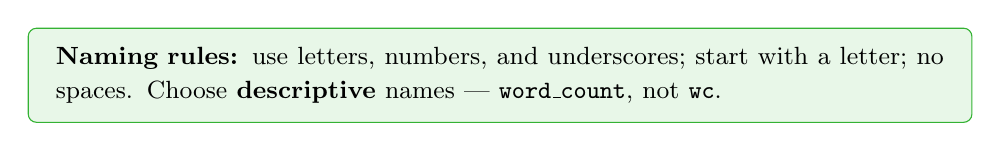
\begin{tikzpicture}
  \node[fill=lightgreen, draw=wurgreen, rounded corners=3pt, inner xsep=10pt, inner ysep=7pt, text width=\textwidth-24pt]{%
    {\small \textbf{Naming rules:} use letters, numbers, and underscores; start with a letter;
    no spaces. Choose \textbf{descriptive} names --- \texttt{word\_count}, not \texttt{wc}.}};
\end{tikzpicture}
\end{frame}

% ── SLIDE 3: data types ──
\begin{frame}{The Basic Data Types}
\vspace{0.2cm}
{\small Every value has a \textbf{type}. The four you'll use constantly:}
\medskip
\begin{center}
\renewcommand{\arraystretch}{1.4}
{\small
\begin{tabular}{p{2.3cm}|p{3.5cm}|p{5cm}}
\textbf{Type} & \textbf{What it is} & \textbf{Example} \\
\hline
\texttt{int} & whole number & \texttt{42}, \texttt{-7}, \texttt{0} \\
\texttt{float} & decimal number & \texttt{3.14}, \texttt{-0.5}, \texttt{2.0} \\
\texttt{str} & text (a ``string'') & \texttt{"hello"}, \texttt{'Python'} \\
\texttt{bool} & true / false & \texttt{True}, \texttt{False} \\
\end{tabular}}
\end{center}
\medskip
{\small You can check any value's type with the \texttt{type()} function:}
\smallskip
\codebox{\textcolor{codeblue}{type}(\textcolor{codeorange}{42})\quad\textcolor{codegray}{\# <class 'int'>}}
\end{frame}

% ── SLIDE 4: numbers and math ──
\begin{frame}{Numbers \& Arithmetic}
\vspace{0.2cm}
{\small Python is a capable calculator. The operators:}
\medskip
\begin{columns}[T]
  \column{0.48\textwidth}\vspace{0pt}
  \codebox{%
  \textcolor{codeorange}{7} \textcolor{codegray}{+} \textcolor{codeorange}{3}\quad\textcolor{codegray}{\# 10  (add)}\\
  \textcolor{codeorange}{7} \textcolor{codegray}{-} \textcolor{codeorange}{3}\quad\textcolor{codegray}{\# 4   (subtract)}\\
  \textcolor{codeorange}{7} \textcolor{codegray}{*} \textcolor{codeorange}{3}\quad\textcolor{codegray}{\# 21  (multiply)}\\
  \textcolor{codeorange}{7} \textcolor{codegray}{/} \textcolor{codeorange}{3}\quad\textcolor{codegray}{\# 2.33 (divide)}}
  \column{0.48\textwidth}\vspace{0pt}
  \codebox{%
  \textcolor{codeorange}{7} \textcolor{codegray}{//} \textcolor{codeorange}{3}\ \textcolor{codegray}{\# 2  (floor div)}\\
  \textcolor{codeorange}{7} \textcolor{codegray}{\%} \textcolor{codeorange}{3}\ \ \textcolor{codegray}{\# 1  (remainder)}\\
  \textcolor{codeorange}{7} \textcolor{codegray}{**} \textcolor{codeorange}{3}\ \textcolor{codegray}{\# 343 (power)}}
\end{columns}
\medskip
{\small\textcolor{midgray}{\textit{Note \texttt{/} always gives a float. \texttt{//} and
\texttt{\%} (``modulo'') are handy more often than you'd expect --- e.g. testing if a number is
even with \texttt{n \% 2 == 0}.}}}
\end{frame}

% ── SLIDE 5: strings ──
\begin{frame}{Working with Strings}
\vspace{0.2cm}
{\small \textbf{Strings} are text, in single or double quotes. You can \textbf{combine} them and
insert variables:}
\medskip
\codebox{%
first \textcolor{codegray}{=} \textcolor{codegreen}{"computational"}\\
second \textcolor{codegray}{=} \textcolor{codegreen}{"text analysis"}\\[6pt]
\textcolor{codegray}{\# join with +}\\
first \textcolor{codegray}{+} \textcolor{codegreen}{" "} \textcolor{codegray}{+} second\quad\textcolor{codegray}{\# "computational text analysis"}\\[6pt]
\textcolor{codegray}{\# f-strings: insert variables with \{\}}\\
\textcolor{codeblue}{f}\textcolor{codegreen}{"I study \{first\} \{second\}"}}
\medskip
{\small \textbf{f-strings} (note the \texttt{f} before the quote) are the modern way to build
text with variables inside --- you'll use them constantly.}
\end{frame}

% ── SLIDE 6: type conversion + input ──
\begin{frame}{Converting Between Types}
\vspace{0.2cm}
{\small Sometimes you need to change a value's type --- e.g. a number typed as text into an
actual number. Use \texttt{int()}, \texttt{float()}, \texttt{str()}:}
\medskip
\codebox{%
\textcolor{codeblue}{int}(\textcolor{codegreen}{"42"})\quad\ \textcolor{codegray}{\# 42   (str -> int)}\\
\textcolor{codeblue}{str}(\textcolor{codeorange}{42})\quad\ \ \ \textcolor{codegray}{\# "42" (int -> str)}\\
\textcolor{codeblue}{float}(\textcolor{codeorange}{3})\quad\ \ \textcolor{codegray}{\# 3.0  (int -> float)}}
\medskip
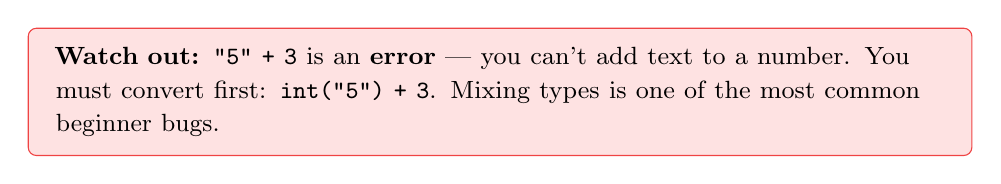
\begin{tikzpicture}
  \node[fill=warnred, draw=warnborder, rounded corners=3pt, inner xsep=10pt, inner ysep=7pt, text width=\textwidth-24pt]{%
    {\small \textbf{Watch out:} \texttt{"5" + 3} is an \textbf{error} --- you can't add text to a
    number. You must convert first: \texttt{int("5") + 3}. Mixing types is one of the most common
    beginner bugs.}};
\end{tikzpicture}
\end{frame}

% ── SLIDE 7: recap ──
\begin{frame}{Module 1: Takeaways}
\vspace{0.3cm}
\begin{itemize}\setlength\itemsep{9pt}
  \item[\textcolor{wurgreen}{\faCheck}] \texttt{print()} displays output; that's your window into what code does
  \item[\textcolor{wurgreen}{\faCheck}] \textbf{Variables} (\texttt{name = value}) hold values under a descriptive name
  \item[\textcolor{wurgreen}{\faCheck}] Four core \textbf{types}: \texttt{int}, \texttt{float}, \texttt{str}, \texttt{bool}
  \item[\textcolor{wurgreen}{\faCheck}] Python does \textbf{arithmetic} with \texttt{+ - * / // \% **}
  \item[\textcolor{wurgreen}{\faCheck}] Build text with \texttt{+} and \textbf{f-strings}; \textbf{convert} types with \texttt{int() float() str()}
\end{itemize}
\medskip
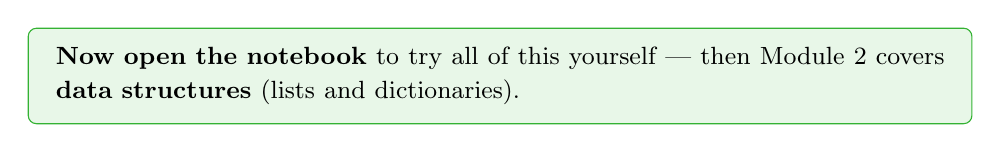
\begin{tikzpicture}
  \node[fill=lightgreen, draw=wurgreen, rounded corners=3pt, inner xsep=10pt, inner ysep=7pt, text width=\textwidth-24pt]{%
    {\small \textbf{Now open the notebook} to try all of this yourself --- then Module 2 covers
    \textbf{data structures} (lists and dictionaries).}};
\end{tikzpicture}
\end{frame}
\end{document}
